\documentclass[letterpaper,titlepage,oneside]{report}
\usepackage[margin=1.0in]{geometry}
\usepackage{graphicx}
\usepackage{float}
\usepackage{caption}
\usepackage{subcaption}
\usepackage{multirow}
\usepackage{booktabs}
\usepackage{tabularx}
\usepackage{todonotes}
\usepackage{hyperref}
\usepackage{amsmath}
\usepackage{pdflscape} 
\usepackage{afterpage}
\usepackage{adjustbox}
\usepackage{array}
%% \usepackage{dcolumn}
%% \usepackage{amsfonts}
%% \usepackage{hyperref}
%% \usepackage{xcolor}
\setlength\parindent{0pt}

\begin{document}

\begin{titlepage}
  \centering
  \vspace*{\fill}
  {\huge\scshape ENPH 257 Lab Report\par}
  \vspace{1cm}
  {\large Brunette, Jacob\quad}
  {\large Fullerton, Dilyn\quad}
  {\large Watt, Ryan\quad}
  {\large Yao, Dickson\par}
  \vspace{1cm}
  {\large Instructor: Dr. Christopher Waltham\par}
  \vspace{1cm}
  {\large \today\par}
  \vspace*{\fill}
  \vfill
\end{titlepage}

\begin{abstract}
  We attempt to estimate several intrinsic thermal properties of a
  brass rod by measuring temperature data during heating and cooling
  and comparing with a simplified one-dimensional model, which
  attempts to account for the effects of conduction, convection,
  and radiation.
  We test the rod under various conditions to observe and characterize
  the effects of orientation, surface quality, and power input on
  the heating behavior and thermal qualities of the rod.
  Thermal parameters are optimized based on the simulation using a
  Levenberg-Marquardt algorithm.
  However, the obtained results carry uncertainty
  values that are too great to be conclusive.
\end{abstract}

\tableofcontents

\chapter{Introduction}
\label{ch:intro}
The purpose of this experiment is to find the parameters that
determine heat transport mechanisms along a brass rod;
these heat transport mechanisms are thermal conduction,
convection and radiation.

\section{Conduction}
Heat diffusion due to conduction is given by the heat equation
\begin{equation}\label{eq:duconduction}
  \left(\frac{\partial}{\partial t}u(\mathbf{r},t)\right)_{\rm{cond}} =
  \frac{k}{c\rho}\nabla^2u(\mathbf{r}, t),
\end{equation}
where $u(\mathbf{r},t)$ is the temperature at position $\mathbf{r}$
and time $t$, $k$ is the thermal conductivity, $c$ is the specific
heat of the material, and $\rho$ is the mass density of the material.

\section{Convection}
Power gain due to convection for a differential surface element
at position $\mathbf{r}$ may be approximated by
\begin{equation}\label{eq:convectionpower}
  P_{\rm{conv}}(\mathbf{r},t) = -k_c\,\delta S(\mathbf{r})
  \left(u(\mathbf{r},t)-u_{\rm{amb}}\right),
\end{equation}
where $k_c$ is the convection coefficient, $\delta S(\mathbf{r})$ is
the differential surface element at $\mathbf{r}$, and $u_{\rm{amb}}$ is
the ambient temperature of the surrounding fluid.
\\\\
Now temperature change due to power for a differential mass element
is given by
\begin{equation}\label{eq:powertodu}
  P = \frac{\partial}{\partial t}Q = c\rho\,\delta V\frac{\partial}{\partial t}u,
\end{equation}
so the rate of change of temperature due to convection is given by
\begin{equation}\label{eq:duconvection}
  \left(\frac{\partial}{\partial t}u(\mathbf{r},t)\right)_{\rm{conv}} =
  -\frac{k_c\,\delta S(\mathbf{r})}{c\rho\,\delta V(\mathbf{r})}
  \left(u(\mathbf{r},t)-u_{\rm{amb}}\right).
\end{equation}

\section{Radiation}
Power gain due to radiation for a differential surface element at
position $\mathbf{r}$ is given by Planck's Law to be
\begin{equation}\label{eq:radiationpower}
  P_{\rm{rad}}(\mathbf{r},t) = -\epsilon\,\sigma\,\delta S(\mathbf{r})
  \left(u(\mathbf{r},t)^4-u_{\rm{amb}}^4\right),
\end{equation}
where $\epsilon$ is the emissivity and $\sigma$ is the Stefan-Boltzmann
constant.
\\\\
Again from Equation (\ref{eq:powertodu}), we can obtain the contribution
to the rate of change of temperature due to radiation
\begin{equation}\label{eq:duradiation}
  \left(\frac{\partial}{\partial t}u(\mathbf{r},t)\right)_{\rm{rad}} =
  -\frac{\epsilon\,\sigma\,\delta S(\mathbf{r})}{c\rho\,\delta V(\mathbf{r})}
  \left(u(\mathbf{r},t)^4-u_{\rm{amb}}^4\right).
\end{equation}

\section{Heat diffusion equation for a cylindrical rod}
For a one-dimensional cylindrical rod of length $L$ and radius
$R$, the heat diffusion equation is 
\begin{equation}\label{eq:heatdiffrod}
  \frac{\partial}{\partial t}u(x,t) =
  \frac{1}{c\rho}\left(
  k\frac{\partial^2}{\partial x^2}u(x, t)
  -k_c\frac{\delta S(x)}{\delta V(x)}
  \left(u(x,t)-u_{\rm{amb}}\right) 
  -\epsilon\,\sigma\frac{\delta S(x)}{\delta V(x)}
  \left(u(x,t)^4-u_{\rm{amb}}^4\right)
  +\frac{P_{\rm{in}}(x,t)}{\delta V(x)}
  \right),
\end{equation}
where $P_{\rm{in}}$ is the power input function.

\chapter{Method}
\label{ch:method}

\section{Experimental setup}
While parts of the apparatus were changed to vary the effects of
heat transfer parameters, the rod remained largely unchanged
throughout the experiment. However, it was necessary to prepare
the brass rod for temperature measurements. A 15 $\Omega$ power
resistor was screwed onto the end of the rod to provide heat.
Thermal paste was dabbed onto the side of the resistor that was
fastened against the rod for more efficient thermal conduction.
Additionally, four holes aligned on the perimeter of the rod were
drilled into one-third of the rod's diameter, where thermocouple
sensors were inserted to sample the temperature at each hole.
The 3 mm holes were evenly spaced 7.25 cm apart, and the hole
nearest to the free end was 1.55 cm from the end of the 33 cm rod.
Additionally, the diameter of the rod was measured to be 2.22 cm
wide. The thermocouples were then numbered in ascending order from
the hole closest to the resistor.
\\

\begin{figure}[ht]
  \centering
  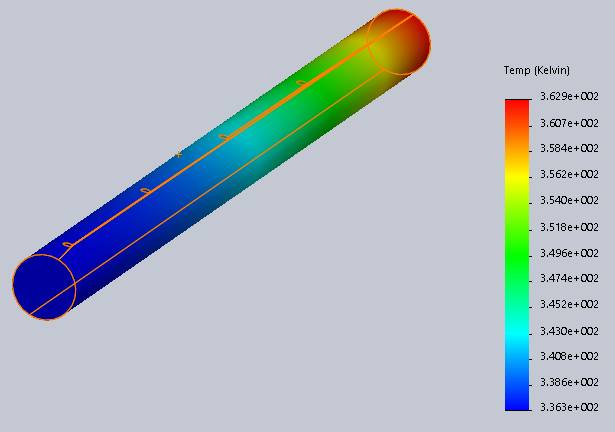
\includegraphics[width=.75\textwidth]{rod}
  \caption{Brass rod CAD design}
  \label{fig:rod}
\end{figure}

The thermocouples are supported by a circuit
(see Figure \ref{fig:circuit}) that amplifies their
signal, which is then read by an Arduino and processed for a
corresponding temperature in MATLAB. Since thermocouples output
a minute voltage, on the scale of millivolts, an instrumental
amplifier is used to amplify the signal. Following amplification,
the output is connected to an inverter to meet the specifications
for the Arduino's analog input, which requires a positive voltage. 
\\\\
The thermocouples are directly connected to the two inputs of a
differential amplifier, with a 10 k$\Omega$ resistor to ground as is
suggested by the manufacturer, with a gain of $\sim$ 1500 to
boost their signal to the scale of several volts, which can be
read by an Arduino. The signal is then fed through a unity
gain inverting operational amplifier so that the signal is
primarily in the positive voltage range. At the output of this
amplifier, there is a low pass filter consisting of a 220 nF
capacitor and a 1 k$\Omega$ resistor to ground. The Arduino
reads data directly from this filter.

\begin{figure}[ht]
  \centering
  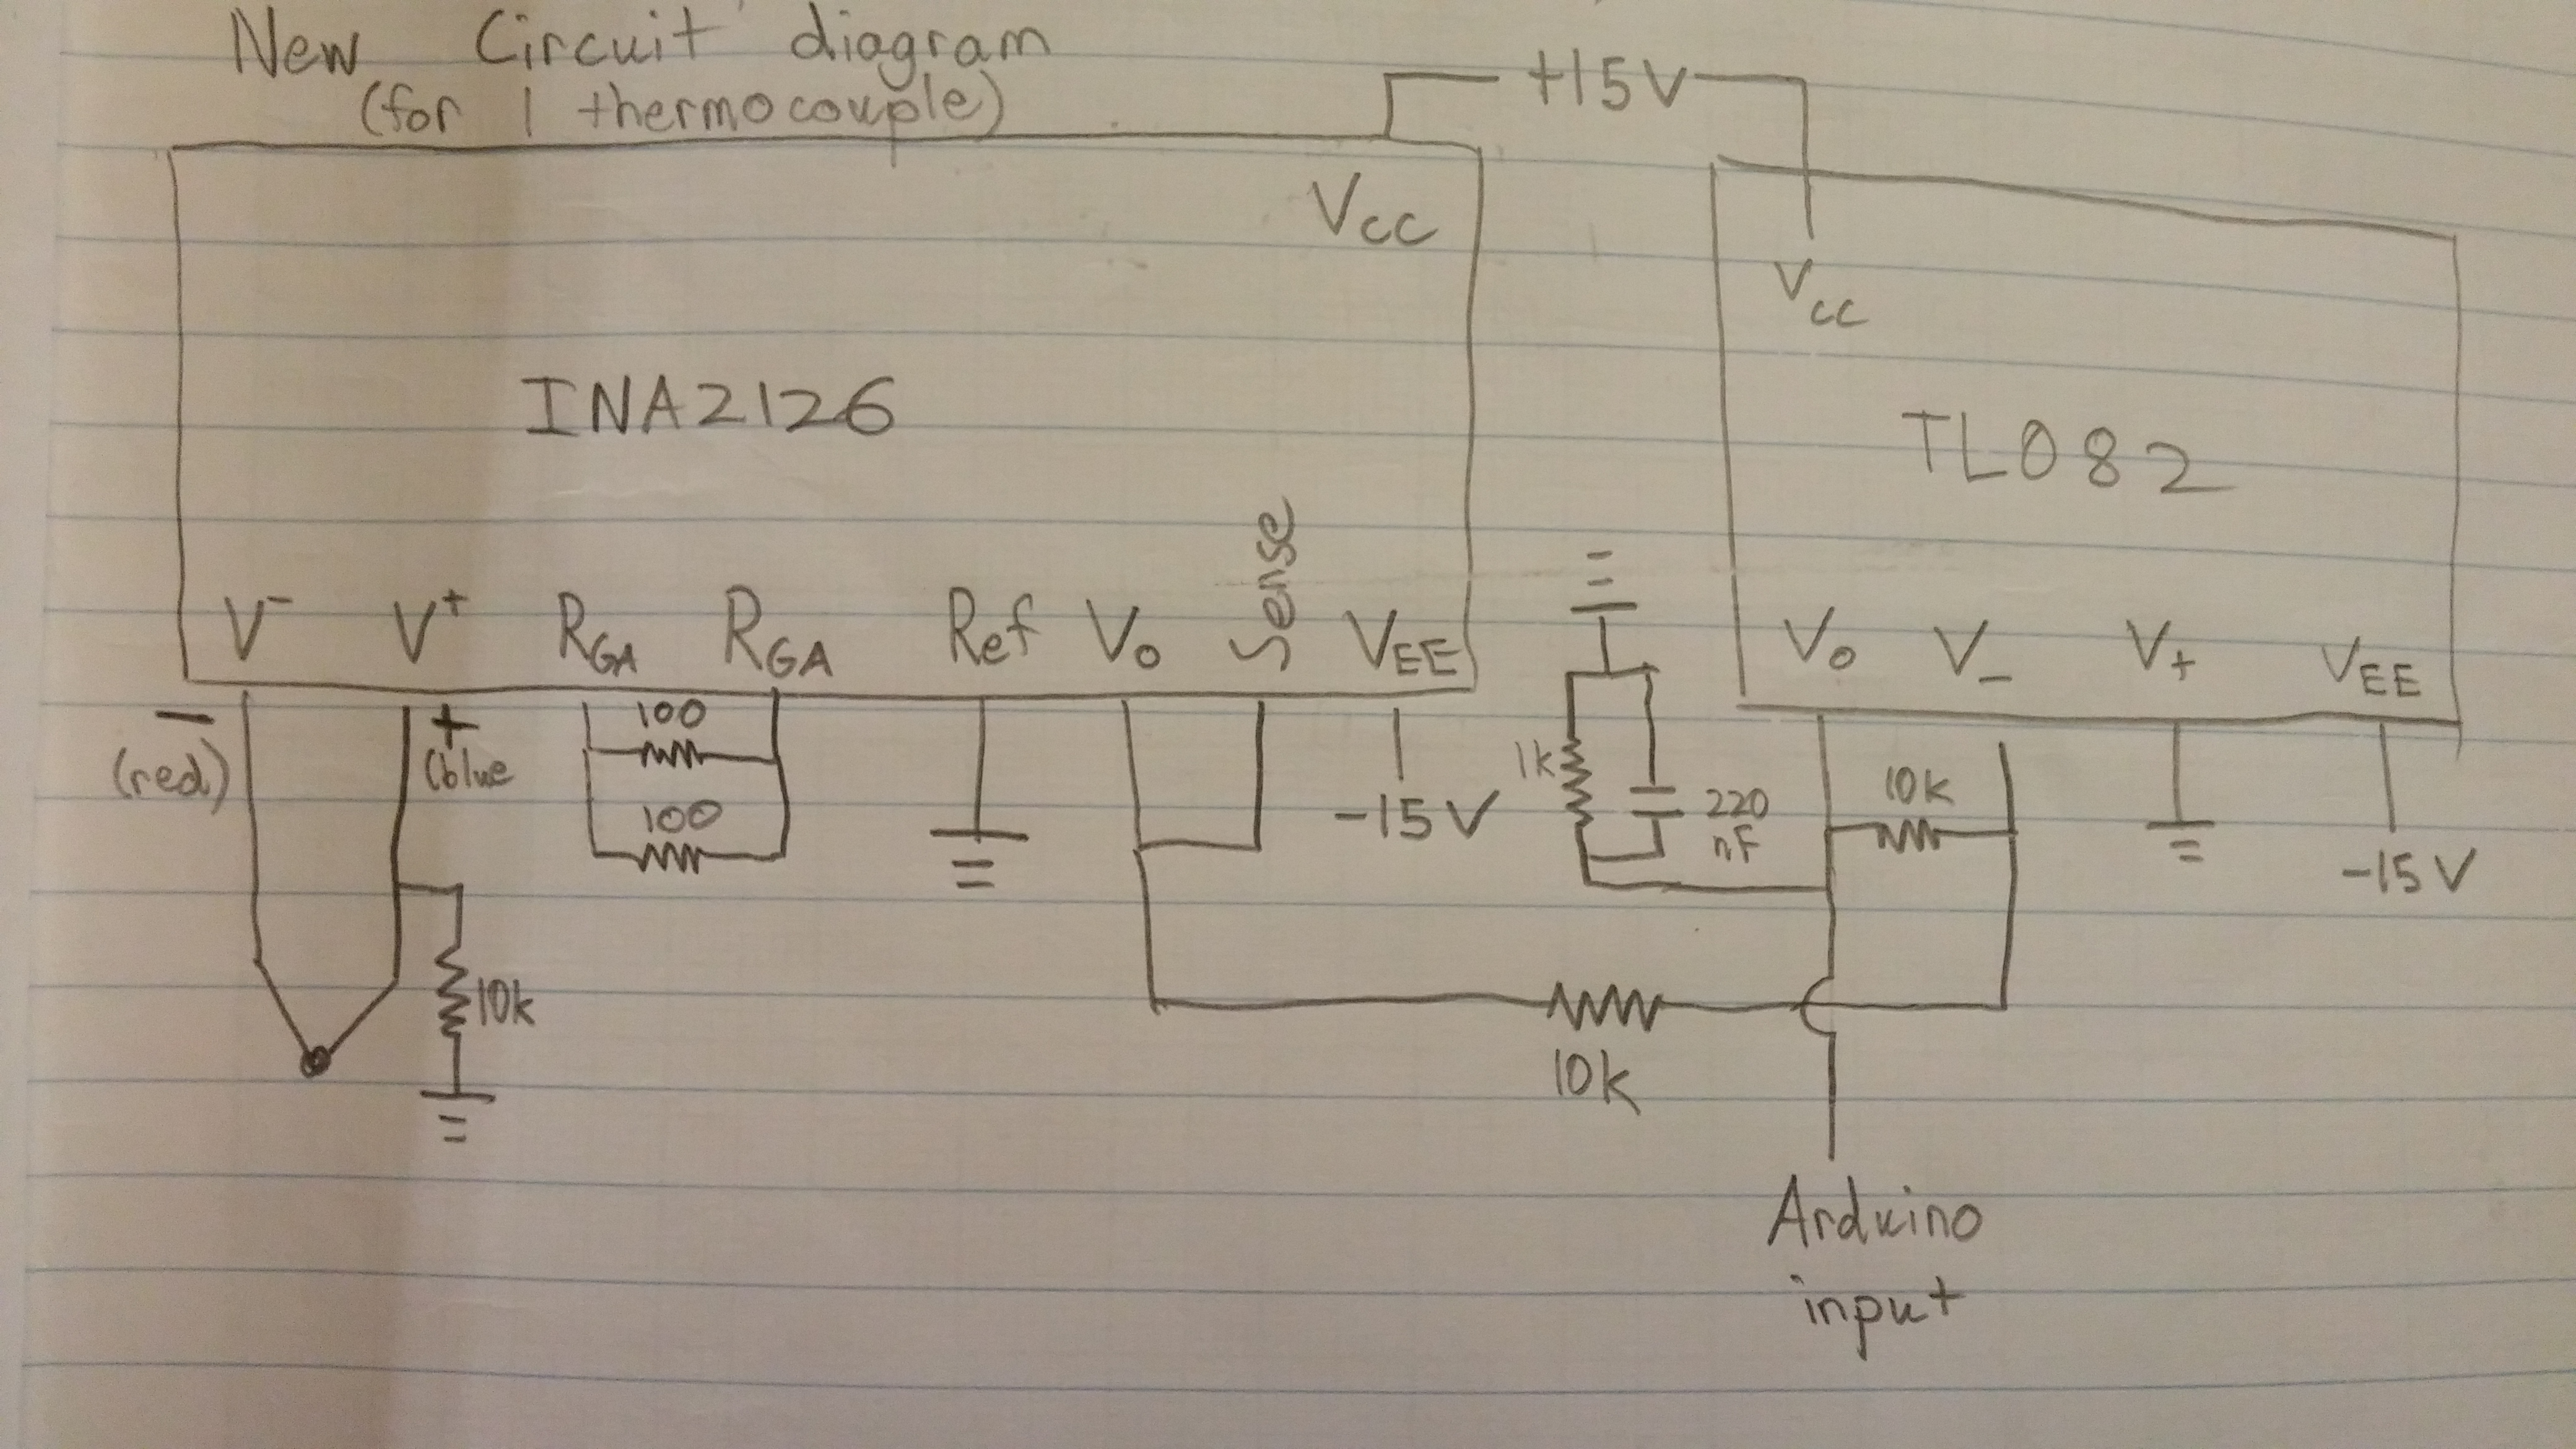
\includegraphics[width=.75\textwidth]{circuit}
  \caption{Thermocouple circuit diagram}
  \label{fig:circuit}
\end{figure}

\section{Calibration}
To find a temperature that corresponds to an analog voltage
reading, a calibration curve was made for each thermocouple.
The thermocouples were placed in a water bath along with a
digital thermometer, and the temperature of the bath was varied
beginning from a hot-water bath at 70$^{\circ}$C, down to around
30$^{\circ}$C as cold water was added. The temperature on the
digital thermometer was manually inputted into a MATLAB program
that recorded the temperature and the voltage that it matched
on each thermocouple. Due to the noisy signal from the
thermocouple voltage, approximately 10 voltage values were
recorded for an individual thermocouple at that temperature,
and averaged. Plotting the temperature-voltage plot over several
temperatures ranging from 30$^{\circ}$ to 70$^{\circ}$C gives a
calibration curve, such as in Figure \ref{fig:calib}.  
Since an approximately linear relationship is observed, a
linear equation converting voltage to temperature was
found for each thermocouple using linear regression.

\begin{figure}[ht]
  \centering
  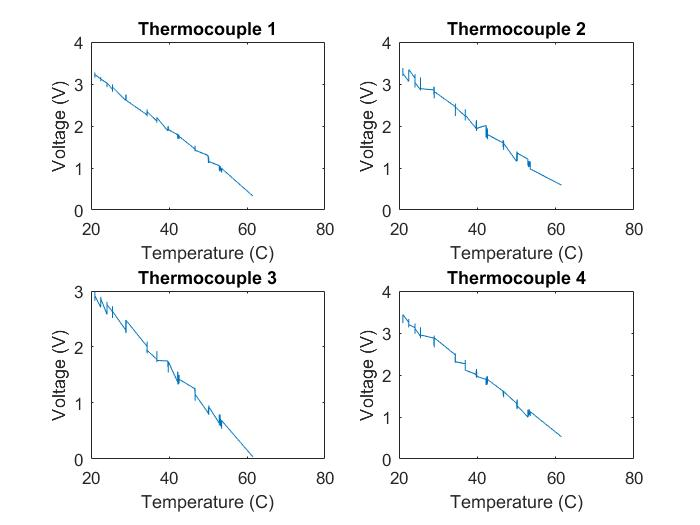
\includegraphics[width=.75\textwidth]{calib}
  \caption{Example calibration curves}
  \label{fig:calib}
\end{figure}

\section{Data aquisition}
Experiments started with collecting the data that determined the
heat transfer coefficients as controlled variables. For the
control group, the rod was set up hanging vertically, clamped
at the end closest to the power resistor. To prevent heat loss
by conduction to the clamps, four rubber O-ring bands were
wrapped around the rod as an insulating buffer between the rod and
clamp. A rough estimate of the desired heating time (to avoid
temperatures over 70$^{\circ}$C) was found using a high-level
simulation. Data collection trials typically ran for one hour,
which included data collection while the rod was both heating and
cooling.

Next, the experimental setup was changed to alter the heat transfer
coefficients. However, multiple experimental trials were run
using one particular setup with several different voltage inputs
to the power resistor for repeated data sets. To vary the
convective coefficient, the rod was placed in three different
positions: horizontally, vertically, and diagonally. In its
horizontal position, the rod was held up by two edges of
a container and tied down with string to restrict its motion.
A stand and ring clamp were used to hold the rod diagonally,
where O-rings were used again to minimize heat loss by
conduction between the rod and clamp. Then, emissivity was
increased by applying black electrical tape over the entire
surface of the rod. Finally, the rod was buffed using sandpaper,
giving it a polished finish to increase its reflectance.
The experiments with varied emissivity had measurements taken in
a vertically clamped position.

\chapter{Simulation and optimization}
\label{ch:simulation}

\section{One-dimensional explicit-step simulation}

The following is the finite difference equation
to simulate heat diffusion based on
Equation (\ref{eq:heatdiffrod}) for a cylindrical rod of
length $L$ and radius $R$. Based on the formalism in
Appendix \ref{ch:finitediff} and supposing x points
$\{x_i:i\in[0,X]\}$ and t points $\{t_n:n\in[0,T]\}$,
the explicit finite difference form
of Equation (\ref{eq:heatdiffrod}) is
\begin{equation}\label{eq:finitediffrod}
  \mathbf{u}^{n+1} = \mathbf{u}^n + \delta t \left(
  \delta\mathbf{u}_{\rm{cond}}^n +
  \delta\mathbf{u}_{\rm{conv}}^n +
  \delta\mathbf{u}_{\rm{rad}}^n +
  \delta\mathbf{u}_{\rm{pow}}^n \right),
\end{equation}
where
\begin{align*}
    \left(\delta \mathbf{u}_{\rm{cond}}^n\right)_i &=
    \frac{k}{c\rho}\cdot\frac{1}{\delta x^2}\cdot
    \begin{cases}
      u_1^n-u_0^n, & \quad i=0\\
      u_{X-1}^n-u_X^n, & \quad i=X\\
      u_{i-1}^n-2u_i^n+u_{i+1}^n, & \quad \text{else}\\
    \end{cases}
    \\
    \left(\delta \mathbf{u}_{\rm{conv}}^n\right)_i &=
    -\frac{k_c}{c\rho}\cdot\frac{\delta S_i}{\delta V_i}
    \left(u_i^n-u_{\rm{amb}}\right)
    \\
    \left(\delta \mathbf{u}_{\rm{rad}}^n\right)_i &=
    -\frac{\epsilon\,\sigma}{c\rho}\cdot\frac{\delta S_i}{\delta V_i}
    \left((u_i^n)^4-u_{\rm{amb}}^4\right)
    \\
    \left(\delta \mathbf{u}_{\rm{pow}}^n\right)_i &=
    \frac{P_i^n}{c\rho\,\delta V_i}
\end{align*}
The differential volume at any point $x_i$ is the same
\begin{equation*}
  \delta V_i = \pi R^2\,\delta x.
\end{equation*}
The exposed surface is different at the ends, however, with
\begin{equation*}
  \delta S_i = 2\pi R\,\delta x +
  \begin{cases}
    \pi R^2, & \quad i=0 \text{ or } i=X\\
    0,       & \quad \text{else}\\
  \end{cases}
\end{equation*}
Finally power input occurs only at one end. It is assumed that
power is a constant $P_1$ during heating and $P_2$ during cooling.
Heating occurs until $t_{\rm{stop}}$ at which point cooling begins.
Thus we have
\begin{equation*}
  P_i^n =
  \begin{cases}
    P_1, & \quad t_0 < t_n < t_{\rm{stop}}\\
    P_2, & \quad t_{\rm{stop}} \leq t_n \leq t_T\\
  \end{cases}
\end{equation*}

\section{Optimization of one-dimensional simulation}
A numerical optimization routine based on the
Levenberg-Marquardt algorithm was used to optimize
thermodynamical parameters by repeatedly varying these parameters,
running the one-dimensional simulation, and comparing the results to
experimental data until optimal parameters were achieved.
This optimization was run for each dataset.
Only the data of the two middle thermocouples was used in the optimization,
as these were generally much better behaved than the edges.
For each optimization, 67 positional points and a time step of .5 seconds
were used. The code used is available at
\url{https://github.com/EmceeEscher/Robot-thermo-group}.

\section{High-level simulation}
SolidWorks was used to produce a CAD file of the rod. Details such as
 the hole placement and depth were included, but O-rings were excluded.
 While, SolidWorks was capable of running a steady-state thermal simulation,
 it seemed inefficient to run a transient-time simulation. Hence,
 the program ANSYS, was used for this purpose instead.
 As a starting point, the material properties of brass, pre-loaded
 into SolidWorks, were selected for the simulation, which set the
 specific heat, conductivity and density. Furthermore, an emissivity
 of 0.03 was found online, and the convective coefficient followed
 a pre-loaded curve in ANSYS, which depended on the difference
 between the temperature of the rod and ambient temperature,
 set to 23.6˚C. Finally, heat flow is simulated to one end of the rod
 with an input value corresponding to the trial we sought to simulate.
\\\\
The heat transfer coefficients that were found through the
optimization program were subsequently inputted to produce a high-level
simulation of the heating of the rod in ANSYS
(see Figure \ref{fig:ansys}). Because additional
parameters such as initial temperature and density were
fitted in the optimization software, a custom material was made
possessing these qualities, and initial conditions were set to
match the parameters.

\chapter{Results}
\label{ch:results}
Results of parameter optimizations are documented in Table
\ref{tab:runsdata}.

\begin{table}[ht]
  \caption{Runs: Descriptions}
  \label{tab:runsdescriptions}
  \centering
  \begin{tabularx}{\textwidth}{|X|r|X|X|}
    \hline
    Run & Potential (V) & Run type & Orientation \\
    \hline
    May  30 - Run 1   &   20.30   &   normal   &    vertical  \\
    May  30 - Run 2   &   17.70   &   normal   &    vertical  \\
    June 01 - Run 1   &   15.18   &   normal   &    horizontal  \\
    June 03 - Run 1   &   10.60   &   normal   &    diagonal  \\
    June 03 - Run 2   &   15.18   &   normal   &    diagonal  \\
    June 06 - Run 1   &   15.18   &   normal   &    vertical  \\
    June 06 - Run 2   &   15.18   &   taped    &    vertical  \\
    June 06 - Run 3   &   20.30   &   taped    &    vertical  \\
    June 08 - Run 1   &   15.18   &   buffed   &    vertical  \\
    June 08 - Run 3   &   20.30   &   buffed   &    vertical  \\
    June 13 - Run 1   &   15.18   &   buffed   &    horizontal  \\
    \hline
  \end{tabularx}
\end{table}

\afterpage{  %% landscape table on next page
  \clearpage
  \thispagestyle{plain}
  \begin{landscape}
    \begin{table}[ht]
    \caption{Runs: Optimization results}
    \label{tab:runsdata}
    \centering
    \newcolumntype{R}{>{\raggedleft\arraybackslash}X}
    \begin{tabularx}{9in}{|X|R|R|R|R|R|R|R|R|R|R|R|}
      \hline
      \textbf{Run} & $\mathbf{k_c}$ & $\mathbf{\epsilon}$ &
      $\mathbf{\rho}$ & $\mathbf{P_1}$ & $\mathbf{P_2}$ &
      $\mathbf{c}$ & $\mathbf{k}$ & $\mathbf{u_0}$
      & $\mathbf{u_{\rm{amb}}}$ &
      \textbf{Power} & \textbf{Power frac}\\
      \hline
      \hline
      \multicolumn{12}{|X|}{\textbf{Vertical}}\\
      \hline
      % vertical data here
      May  30 - Run 1   &   12.5668   &   1    &   8782.77   &   25.0745   &   -1.9987   &   382.1010   &   100.0   &   295.8740   &   304.3108      &   27.47267   &   0.9127      \\
      \hline
      May  30 - Run 2   &    8.1040   &   1    &   8293.50   &   20.8860   &    0.0707   &   361.0000   &   100.0   &   301.8020   &   298.6727      &   20.88600   &   1.0000      \\
      \hline
      June 06 - Run 1   &    8.4069   &   1    &   8493.26   &   13.9178   &    0.9902   &   369.6951   &   100.0   &   297.6903   &   297.1670      &   15.36216   &   0.9060      \\
      \hline
      June 06 - Run 2   &   19.1927   &   0    &   8370.07   &   15.3622   &    3.3211   &   364.3329   &   100.0   &   300.8075   &   294.2197      &   15.36216   &   1.0000      \\
      \hline
      June 06 - Run 3   &   15.5571   &   1    &   8447.59   &   26.6469   &    2.5599   &   367.7051   &   100.0   &   300.8720   &   296.5346      &   27.47267   &   0.9699      \\
      \hline
      June 08 - Run 1   &    4.7554   &   1    &   8293.50   &   12.9929   &   -0.0267   &   361.0000   &   102.9   &   298.7773   &   296.1117      &   15.36216   &   0.8458      \\
      \hline
      June 08 - Run 3   &    6.9179   &   1    &   8452.08   &   21.8658   &   -0.5948   &   367.8965   &   100.0   &   300.3236   &   301.7212      &   27.47267   &   0.7959      \\
      \hline
      \textbf{Mean}     &   10.7858   &        &             &             &             &              &           &              &                 &              &               \\
      \hline
      \textbf{Std Dev}  &    5.1767   &        &             &             &             &              &           &              &                 &              &               \\
      \hline
      \hline
      \multicolumn{12}{|X|}{\textbf{Horizontal}}\\
      \hline
      % horizontal data here
      June 01 - Run 1   &   05.9338   &   1    &   8603.09   &   13.1600   &   -0.9993   &   370.2600   &   100.0   &   296.9922   &   301.6543      &   15.36216   &   0.8567      \\
      \hline
      June 13 - Run 1   &   08.7668   &   1    &   8718.01   &   15.3622   &   -0.0000   &   379.9838   &   100.0   &   298.1978   &   300.2710      &   15.36216   &   1.0000      \\
      \hline
      \textbf{Mean}     &    7.3503   &        &             &             &             &              &           &              &                 &              &               \\
      \hline
      \textbf{Std Dev}  &    2.0032   &        &             &             &             &              &           &              &                 &              &               \\
      \hline
      \hline
      \multicolumn{12}{|X|}{\textbf{Diagonal}}\\
      \hline
      % diagonal data here
      June 03 - Run 1   &   05.8893   &   1    &   8729.63   &   07.4374   &   -0.0149   &   380.0648   &   100.0   &   297.2276   &   297.7102      &   07.49067   &   0.9929      \\
      \hline
      June 03 - Run 2   &   07.3700   &   1    &   8537.28   &   15.2304   &   -0.1991   &   371.9972   &   100.0   &   299.6723   &   299.9362      &   15.36216   &   0.9914      \\
      \hline
      \textbf{Mean}     &    6.6296   &        &             &             &             &              &           &              &                 &              &               \\
      \hline
      \textbf{Std Dev}  &    1.0470   &        &             &             &             &              &           &              &                 &              &               \\
      \hline
      \hline
      \multicolumn{12}{|X|}{\textbf{TOTALS}}\\
      \hline
      % averages
      \textbf{Mean}     &             & 0.9091 &   8520.07   &             &             &   370.5488   &   100.3   &   298.9306   &   298.9372      &              &   0.9338      \\
      \hline
      \textbf{Std Dev}  &             & 0.3015 &    171.77   &             &             &     7.4300   &     0.9   &     1.9007   &     2.9581      &              &   0.0743      \\
      \hline
    \end{tabularx}
    \end{table}
  \end{landscape}
  \clearpage
}

\chapter{Analysis}
\label{ch:analysis}

\section{Quality of optimization}

\subsection*{Individual fits}
Table \ref{tab:optindividual} describes the quality of the individual fits to
data from which individual thermodynamical parameters were derived.
The slope and intercept are those of the linear regression and should
theoretically be 1 and 0 respectively. The R$^2$ is the square of the
correlation coefficient between the simulation and experimental data; a value
close to 1 indicates a strong fit. Finally standard error is the standard
error of the estimates of slope and intercept.

\begin{table}[ht]
  \caption{Optimization quality: Individual fits}
  \label{tab:optindividual}
  \centering
  \begin{tabularx}{0.75\textwidth}{|X|r|r|r|r|r|}
    \hline
    Run & Slope & Intercept & R-squared & Std Err \\
    \hline
    May  30 - Run 1   &   0.9998   &   0.0558   &    0.9956   &   0.0010 \\
    May  30 - Run 2   &   1.0635   & -19.7122   &    0.9193   &   0.0041 \\
    June 01 - Run 1   &   0.9999   &   0.0251   &    0.9964   &   0.0009 \\
    June 03 - Run 1   &   1.0000   &   0.0110   &    0.9969   &   0.0005 \\
    June 03 - Run 2   &   0.9999   &   0.0298   &    0.9973   &   0.0005 \\
    June 06 - Run 1   &   0.9999   &   0.0257   &    0.9942   &   0.0010 \\
    June 06 - Run 2   &   1.0056   &  -1.7206   &    0.9912   &   0.0010 \\
    June 06 - Run 3   &   0.9997   &   0.1019   &    0.9826   &   0.0014 \\
    June 08 - Run 1   &   0.9999   &   0.0205   &    0.9986   &   0.0005 \\
    June 08 - Run 3   &   0.9998   &   0.0594   &    0.9971   &   0.0006 \\
    June 13 - Run 1   &   1.0028   &  -0.8647   &    0.9966   &   0.0006 \\
    \hline
  \end{tabularx}
\end{table}

\subsection*{Average fits}
Based on the average values determined in Table \ref{tab:runsdata},
simulations were run for each trial where the global average values
were used for ${\epsilon}$, ${\rho}$, ${c}$, and ${k}$.
Average values for the particular geometry were used for $k_c$. And
specific values were usedfor ${P_1}$, ${P_2}$, ${u_0}$,
and ${u_{\rm{amb}}}$, as these are heavily dependent on the particulars
of the trial.

\begin{table}[H]
  \caption{Optimization quality: Average fits}
  \label{tab:optavg}
  \centering
  \begin{tabularx}{0.75\textwidth}{|X|r|r|r|r|r|}
    \hline
    Run & Slope & Intercept & R-squared & Std Err \\
    \hline
    May  30 - Run 1   &   0.1915   & 246.1704   &    0.4222   &   0.0034 \\
    May  30 - Run 2   &   0.3282   & 202.8493   &    0.7470   &   0.0025 \\
    June 01 - Run 1   &   0.2619   & 223.4058   &    0.4569   &   0.0043 \\
    June 03 - Run 1   &   0.3522   & 192.5934   &    0.7374   &   0.0019 \\
    June 03 - Run 2   &   0.2800   & 217.0452   &    0.6371   &   0.0022 \\
    June 06 - Run 1   &   0.3420   & 195.1229   &    0.6018   &   0.0035 \\
    June 06 - Run 2   &   0.2935   & 209.0217   &    0.8326   &   0.0014 \\
    June 06 - Run 3   &   0.2691   & 216.8487   &    0.8205   &   0.0013 \\
    June 08 - Run 1   &   0.4113   & 174.5721   &    0.6152   &   0.0042 \\
    June 08 - Run 3   &   0.2540   & 229.4468   &    0.4798   &   0.0028 \\
    June 13 - Run 1   &   0.2650   & 221.1282   &    0.5807   &   0.0023 \\
    \hline
  \end{tabularx}
\end{table}

\subsection*{High Level Simulation Results}
The results of the high-level simulation are comparable to the
experimental data gathered on June 6th, which used 15.18 V
to the power resistor and 15.36 W of heating power, and was set
up vertically, prior to being polished. For thermocouples 2 to
4, the temperatures after a 1200 second heating period have
approximately a 3$^{\circ}$C difference to the simulation.
This demonstrates that the parameters derived from the fitting
optimization produced plausible (although not completely
accurate) values.

\begin{figure}[ht]
  \centering
  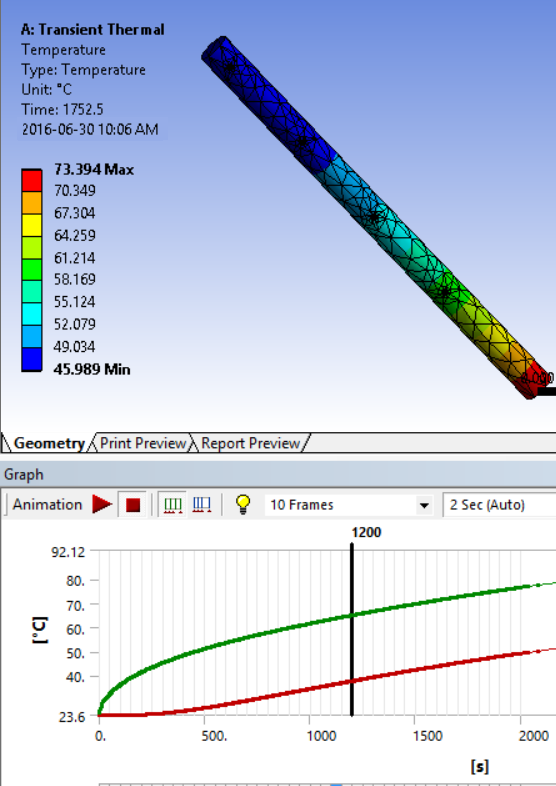
\includegraphics[width=.5\textwidth]{ansysrod}
  \caption{Initial ANSYS simulation 7.5 V}
  \label{fig:ansysrod}
\end{figure}

\begin{figure}[ht]
  \centering
  \begin{subfigure}[h]{0.4\textwidth}
    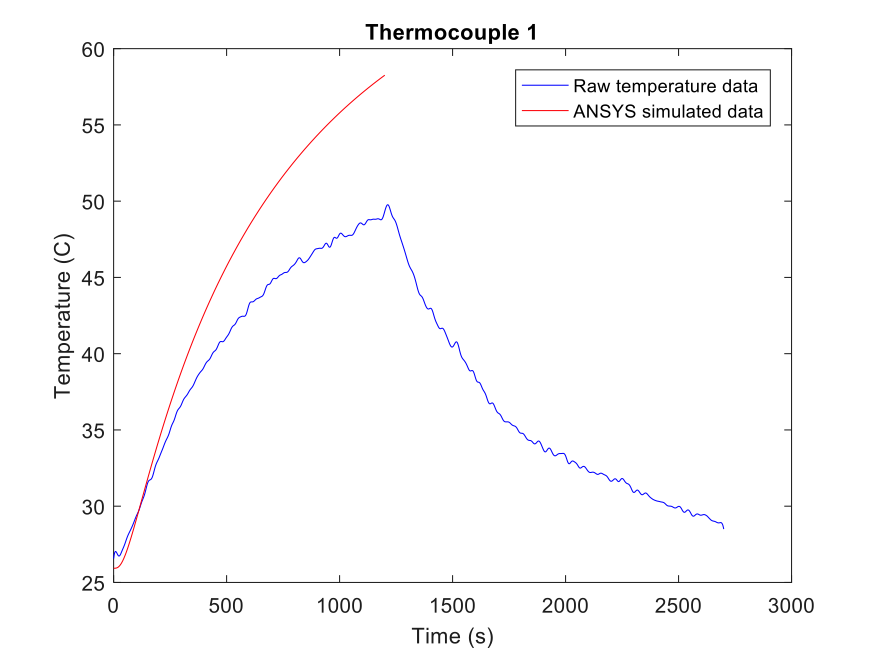
\includegraphics[width=1\textwidth]{ansys1}
    %% \caption{ANSYS simulation for thermocouple 1}
  \end{subfigure}
  \quad
  \begin{subfigure}[h]{0.4\textwidth}
    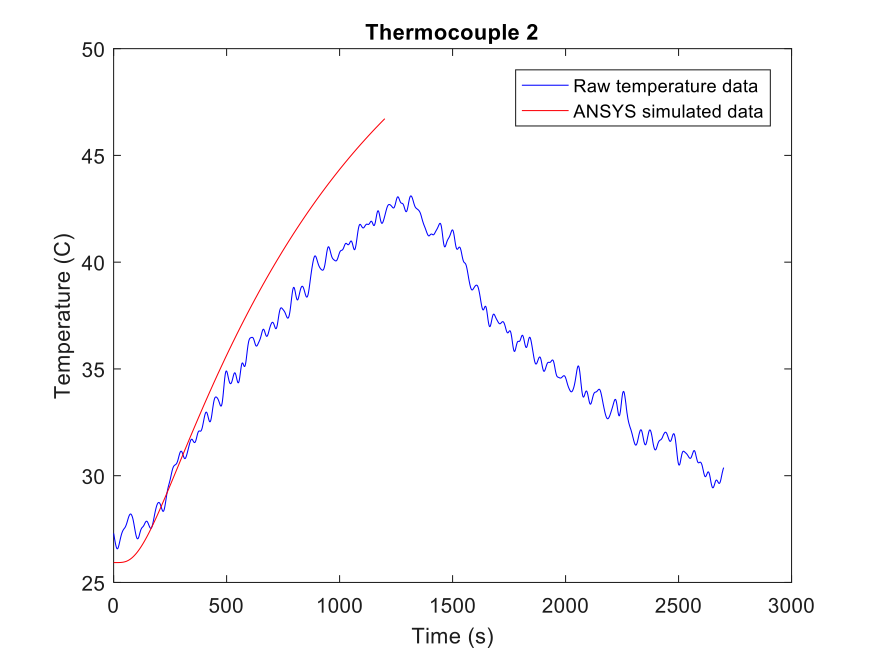
\includegraphics[width=1\textwidth]{ansys2}
    %% \caption{ANSYS simulation for thermocouple 2}
  \end{subfigure}
  \\
  \begin{subfigure}[h]{0.4\textwidth}
    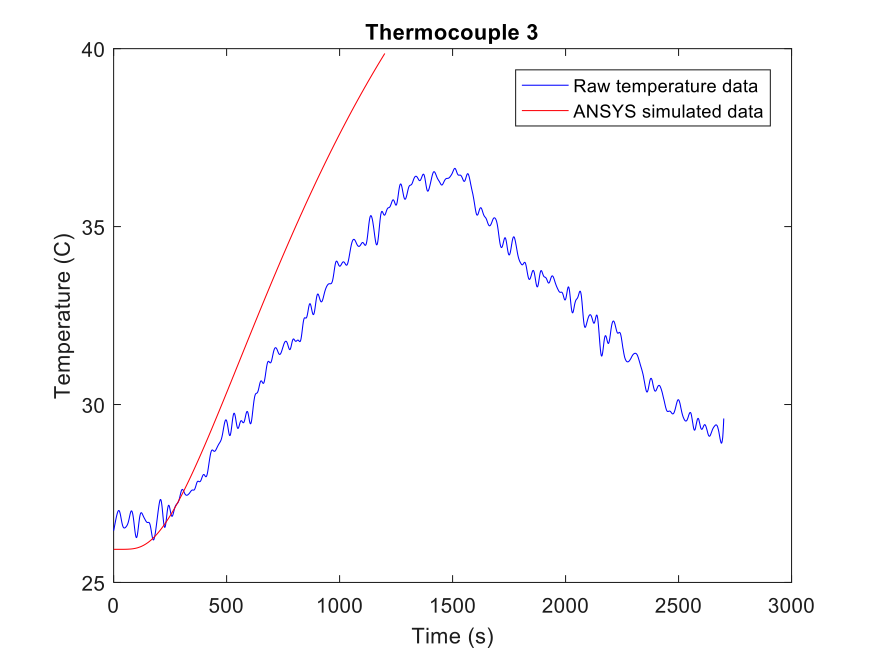
\includegraphics[width=1\textwidth]{ansys3}
    %% \caption{ANSYS simulation for thermocouple 3}
  \end{subfigure}
  \quad
  \begin{subfigure}[h]{0.4\textwidth}
    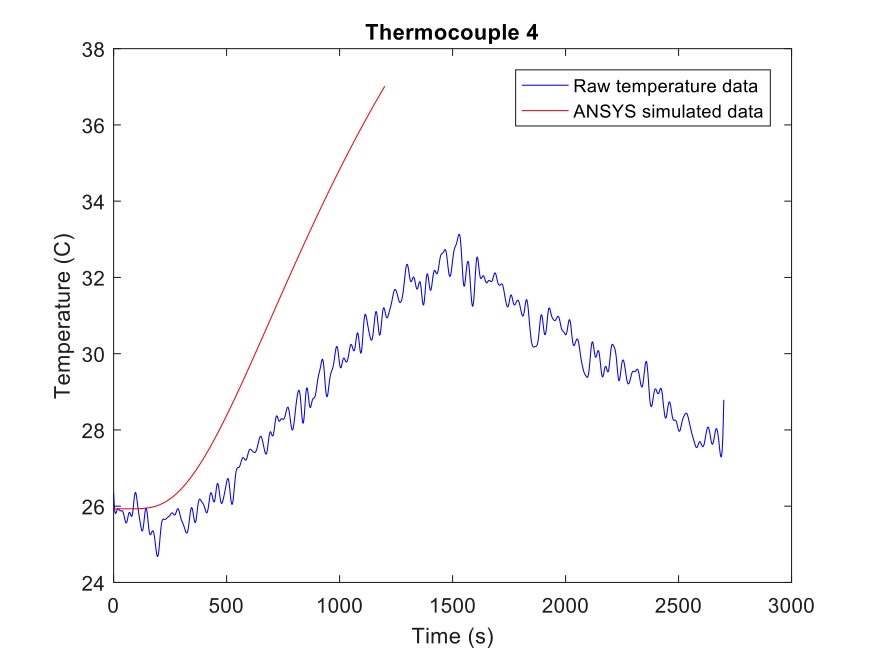
\includegraphics[width=1\textwidth]{ansys4}
    %% \caption{ANSYS simulation for thermocouple 4}
  \end{subfigure}
  \caption{Example ANSYS simulation results for thermocouples 1-4}
  \label{fig:ansys}
\end{figure}

\section{Explanation of results}

\subsection* {Convective heat transfer coefficient}
Our values for the convective heat transfer coefficient had a
large range of values (up to 77.5\% of the average); thus it is
almost meaningless beyond finding the correct order of
magnitude of the actual result.
A large part of the difficulty in determining $k_c$ is that it is
affected by many different variables beyond just geometry,
and treating it as a constant is a major approximation.
We did not sufficiently isolate the geometry as the only variable
affecting $k_c$, so we were not able to determine its actual value
to any degree of certainty.

\subsection* {Emissivity}
Although in accordance with Table (\ref{tab:runsdata}) our average
value is at 0.91, this does not reflect the
actual value of the rod. This is due to the optimization
consistently hitting its upper bound of 1.0 and on one
occasion reaching its lower bound of 0.
These occurrences did not line up with the application of taping
or buffing the rod and so we consider our values to be inherently
flawed.

\subsection* {Density}
The simulation's derived density has no physical relevance as we
measured it to be 7971 kg/m$^3$. Additionally, the simulation had
no way to directly calculate the density as it only ever
appeared multiplied by the specific heat.
In hindsight, the value of density should have been measured early on
so as to input the measured value for density instead of
letting the program try to fit it.

\subsection* {Power2}
This value represents the power loss from the resistor when the rod
was cooling. The resistor significantly changed the properties
of the end of the rod it was connected to, and we attempted to
account for its effect by allowing it to having a negative power
input during the cooling period, independent of the heating power.
This allowed strong fitting of the full heating/cooling period;
however the program sometimes fit an exceedingly large value
(or even a positive value) to this power draw,
indicating that this model is not likely physically accurate.

\subsection* {Specific heat}
The value for specific heat averages to 370 J/g*K,
which is a reasonable value with low relative error.
A potential issue comes from the fact that its simulation value
occasionally reached the imposed lower bound of 361; however,
this did not occur frequently enough to shift our bounds on
its actual value too far from this average.
Therefore, we consider this value to have an uncertainty of 20 J/g*K.

\subsection* {Thermal Conductivity}
This value was seen to consistently hit its imposed lower bound of
100 W/m*K in the optimization which tells us most likely that
its proper value is well below 100, although no specific
numerical approximation can be made with this data.

\subsection* {$u_0$ and $u_{\rm{amb}}$}
Instead of manually inputting the starting temperature of the rod
and the room, we let the program attempt to optimize for temperatures
that led to the best fit of the data. The program generally did a
good job of optimizing for a starting temperature and an ambient
temperature that were physically reasonable, but it was an
unnecessary exercise, and it would have been
a better idea to measure these values and input them into the
simulation manually, instead of forcing the program try to
optimize them.

\subsection* {Power Fraction}
The average value of power fraction was found to be 93\% which
is a reasonable value in this scenario. The simulation frequently
placed values under its imposed maximum bound of 100\% for this
value, and so we assign it an uncertainty of 10\%.

\section{Uncertainty}

\subsection*{Lab setup}

\subsubsection*{Thermocouple fluctuations (key source)}
Thermocouple readings fluctuated a lot, despite the fact that
we fed them into both an instrument amplifier and an op-amp
inverter circuit before we tried to do any kind of filtering.
Our filtering was effectively a simple low-pass filter which,
in practice, did very little. Consequently, consecutive
readings of temperatures (converted from the thermocouple
voltage readings) had large uncertainties, as they regularly
fluctuated with a range of $\pm$2$^{\circ}$C for readings taken
half a second apart. We tried to smooth out the noise in our data
with MATLAB's smoothing functionality, but even the smoothed
data had frequent spikes. This had a large effect on all of
our future efforts at fitting parameters to the data.

\subsubsection* {Heat loss of power resistor}
The end of the rod with the power resistor had different
physical conditions (especially emissivity) than the rest of
the rod. Obviously, it was a heat source when plugged in,
but it became a heat sink when we unplugged it and allowed the rod
to cool. During cooling, the end of the rod closest to the
resistor often dropped to lower temperatures than the rest of
the rod, most likely due to the presence of the resistor.
We attempted to model this in our simulation, using
a \texttt{power2} parameter to represent of the power lost through
the resistor while the rod was cooling. This added another
parameter that we needed to fit, however, and possibly made the
finite difference model we used into a poorer representation of
the physical state of the rod.

\subsubsection* {Lack of multiple trials:}
Due to time constraints, we were unable to run multiple trials
for most of our data collection setups, which increased the
uncertainty in our data and hampered our ability to catch and
correct experimental mistakes. This was especially detrimental
to the convective heat transfer coefficient result,
which depends the most upon particular experimental setups. 

\subsection*{Simulation and optimization}

\subsubsection*{Errors in simulation}
The simulation is subjected to certain errors based on the approximations
of the finite differencing scheme (see Appendix \ref{ch:finitediff}).
Error in position (Equation (\ref{eq:expliciterrdx})) is quadratic, and since
the simulations used $\delta x = 0.005$ m, the error in the spatial
derivative is on the order of $10^{-5}$ m and thus largely negligible.
Error in time (Equation (\ref{eq:expliciterrdt})) is linear, and since
the simulations used $\delta t = 0.25$ s, the error in the time derivative
is on the order of $0.1$. While the condition for numerical stability
(Equation (\ref{eq:stability})) is
satisfied, this certainly could have contributed to the
error in the final optimized parameter, especially since only a rudimentery
explicit scheme was used. Perhaps it would have been useful to implement
an implicit scheme, which is guaranteed to be numerically stable, or a
a Crank-Nicolson scheme, which is guaranteed to be numerically stable and
in which the error in time is quadratic.
Alternatively, a smaller time step could have been used, albeit this would
have made optimization extremely slow.

\subsubsection*{Errors in optimization}
Errors in the optimization setup are difficult to quantify, but probably
quite influencial here. The Levenberg-Marquardt algorithm is guaranteed
to reach the local minimum within the set boundaries, and having set
many different starting values with no effect on the results, it is quite
evident that issues in the final results are not being caused by a failure
of the algorithm to converge to the global minimum within the boundaries.
Rather the most likely failure of the optimization procedure was overfitting.
Namely, since the optimization was allowed to vary so many parameters, the
individual parameters of interest were decoupled from the final results
and only their relative values were fixed. This idea is expanded upon in
\nameref{sec:emiss}.

\subsection*{Emissivity}
\label{sec:emiss}
The intent of the experiment was to measure the emissivity of the
rod in three different states: unaltered condition,
covered with electrical tape, and buffed to be as shiny as possible.
Our expectation was that these three states would each cause
a distinct emissivity, with the taped rod having a higher
emissivity and the buffed rod having a lower emissivity.
This was not made evident by the data. Every run of our
simulation optimization program resulted reaching the boundaries
(either 0 or 1). The actual state of the rod had little to no
effect on which of these two results were produced;
the starting value we gave the optimization program tended to have
more of an influence.
\\\\
We believe that these aberrant results were due to either the design
of the model or overfitting. In either case, the effect of the
parameter had a negligible effect on the quality of the optimization,
resulting in it consistently being fully maximized or minimized.
In the eyes of the program the terms $\sigma(u(x,t)^4-u_{\rm{amb}}^4)$
and $(u(x,t)-u_{\rm{amb}})$ are roughly of the same magnitude,
and so it arbitrarily balances $\epsilon$ with $k_c$. Because the
radiation term does tend to be bigger, it ends up 
maximizing $\epsilon$ and minimizing $k_c$. This unstable balanced is only
halted by the manually imposed boundary on $\epsilon$ at 1
(the maximum physically possible). If we leave it unbounded,
the program tends to increase $\epsilon$ and bring $k_c$ to almost 0,
because it is easier to optimize with just the one necessary term.
Because we were unable to get any realistic values of emissivity,
we decided that it would be better to state this fact than try to
come up with an arbitrary uncertainty for a value that is
obviously physically wrong.

\subsection*{Specific heat}
Error Sources:
\begin{itemize}
\item Constant multiplication by mass density which was left variable
\item Likely constant offset as density bounds did not include measured value
\item The inverse has a linear relationship with the time derivative
\end{itemize}
Specific heat measurements yield a value with low relative error;
however, error must still be accounted for, as there were multiple
relevant sources. The primary source that may have affected
the accuracy of our measurement is the fact that our measured
mass density is lower than all of our simulation's calculated mass
densities. (The minimum bound for mass density in the simulation
was above the measured value). As these two values are always
multiplied by one another for all terms in the temperature
time-derivative model, this would lead to a lower value for the
specific heat to account for the higher value for density.
Furthermore, as the mass density was allowed to vary between
simulation runs, unnecessary uncertainty was induced into the
specific heat, as only their product mattered in the model.
Another consideration for the specific heat's error is that its
inverse is a linear factor of the heat exchange derivative and
so any other linear effects over the rod, which would be
accounted for in more complex models, could only be accounted
for by varying the mass density and specific heat in the simulation.

\subsection*{Power fraction}
Error sources:
\begin{itemize}
\item Heat loss from resistor is temperature dependent
\item Rubber bands near power resistor 
\item Positive note, never exceeded actual value
\end{itemize}
One key issue is that the heat loss out of the power resistor
into the environment, which is a portion that would not be
transmitted to the rod and is dependent on the temperature of the
power resistor for convection as well as radiation.
The simulation model did not account for this, as it assumed
that the power transmitted to the rod remained constant for the
duration of the heating period. However, attempting to calculate
this would have introduced the new variables of the power
resistor's emissivity and convection coefficient which would
have given the simulation further degrees of freedom and increased
complexity of data verification and analysis.
Another potential issue is the potential for power losses out
through the rubber bands near the power resistor. As we had no
thermocouples between the power resistor and the rubber bands
any losses of power due to these could be seen as equivalent to
power losses in transmission from the power resistor.
On a positive note, however, the power fraction never went above
1 and so the simulation at the very least never over-estimated
the power sent down the rod.

\subsection*{Convection coefficient}
While properties of the rod and air, most of which are constant,
must be used to calculate a convective coefficient, the temperature
difference between the rod and air also contributes to the value
of the convective coefficient. Thus, as voltage input and heating
power varied the rate of change in temperature for the rod in
different experimental trials, the convective coefficients found
vary accordingly. Despite the fact that the values of
convective coefficients follow a logarithmic curve such that
the rate of change of these values decrease as the
temperature difference between the air and the rod increases,
it was impactful to the results of the experiment.
The convective coefficients could also be affected by airflow
in the lab (such as currents caused by people walking past the
lab setup). 

\subsection*{Thermal conductivity}
While the variation in the conductivity parameter is very low due
to the poor choice of optimization boundaries (the conductivity almost
always hit the lower bound that we set), it is expected that the
true measured value of conductivity would have varied by the
influence of several physical factors. Holes made for temperature
sensors disrupt the flow of heat along the rod and influence
heat transfer. While rubber O-rings were selected for their
low conductivity, their contact with the rod may have allowed
for additional heat loss as well. Lastly, contact was made with
the rod by experimenters on several occasions throughout the
experiment to ensure proper heating, which also slightly
contributes to uncertainty. 

\chapter{Conclusion and Summary}
\label{ch:conclusion}
The goal of this experiment was to determine the thermal
conductivity, specific heat capacity, emissivity, and convective
heat transfer coefficient of a rod, as well as the fraction
of power generated by a power resistor that flowed down the rod,
and to observe how these values change with
the orientation and color of the rod.
\\
We obtained the following numerical results:
\begin{description}
\item [Thermal conductivity:] 100.26 W/mK
\item [Specific heat capacity:] 370.55 $\pm$ 20 J/gK
\item [Power fraction:] 93.38\% $\pm$ 10\%
\item [Emissivity:] 0.9091 W/m$^2$ (not observed to change with different colored rod)
\item [Convective heat transfer coefficient:]\hfill
  \begin{itemize}
  \item Vertical: 8.40 W/m$^2$K
  \item Horizontal: 5.66 W/m$^2$K
  \item Diagonal: 6.63 W/m$^2$K
  \end{itemize}
\end{description}

Overall, the obtained data was severly inconsistent and uncertain,
and it is difficult to draw meaningful conclusions from our
numerical results. Indeed, for many of the results, uncertainties
could not even be assigned,
as rigrously establishing bounds would be implausible.
\\\\
It is suspected that this was due to a number of factors, most
notably noise in the directly-measured temperature data and
methodology used to estimate parameters from the temperature data.
Possible improvements to the experimental procedure might include
developing a better way to shield noise in temperature measurements,
creating more sophisticated simulation and optimization techniques,
and reducing the number of degrees of freedom the optimization has to
account for by making more physical measurements.

\appendix

\chapter{Group member roles}

\begin{table}[ht]
  \caption{Group member roles}
  \label{tab:roles}
  \centering

  \newcolumntype{R}[2]{%
    >{\adjustbox{angle=#1,lap=\width-(#2)}\bgroup}%
    l%
    <{\egroup}%
  }
  \newcommand*\rot{\multicolumn{1}{R{90}{1em}|}}

  \begin{tabularx}{.75\textwidth}{|X|c|c|c|c|c|c|c|c|c|}
    \hline
    Member &
    \rot{Exp. Design} &
    \rot{Exp. Construction} &
    \rot{DAQ Elec.} &
    \rot{DAQ Code} &
    \rot{Simulation} &
    \rot{SolidWorks} &
    \rot{Data analysis} &
    \rot{Results synthesis} &
    \rot{Writing} \\
    \hline
    Brunette, Jacob    &    &    &    &    &    &    &    &    &    \\
    \hline
    Fullerton, Dilyn   &  0 &  0 &  0 & 50 & 95 &  0 & 20 & 20 & 30 \\
    \hline
    Watt, Ryan         &    &    &    &    &    &    &    &    &    \\
    \hline
    Yao, Dickson       &    &    &    &    &    &    &    &    &    \\
    \hline
  \end{tabularx}
\end{table}

\chapter{Explicit Method of Finite differencing}
\label{ch:finitediff}
The following is a description of the explicit method of
finite differencing, demonstrated
using the simple example of the one-dimensional heat conduction equation
\begin{equation}\label{eq:condsimp}
  \frac{\partial}{\partial t}u(x,t) = \alpha\frac{\partial^2}{\partial x^2}u(x,t).
\end{equation}

\section*{Finite difference equation}
In the explicit method for finite differencing, the temperature for
each spatial point can be independently determined from the previous
step. That is,
\begin{equation}\label{eq:explicit}
  u_i^{n+1} = u_i^n + \alpha\cdot\frac{\delta t}{\delta x^2}\cdot
  \left(u_{i-1}^n - 2u_i^n + u_{i+1}^n\right),
\end{equation}
where the superscript $n \in [0, T]$ signifies the step in time
$t_n$ and the
subscript $i \in [0, X]$ represents the position
$x_i$. $\delta t$ and $\delta x$
are the time steps in time and position respectively.
\\\\
If we define
\begin{equation*}
  \zeta = \alpha\cdot\frac{\delta t}{\delta x^2},
\end{equation*}
then this can be written as a linear relationship
\begin{equation}\label{eq:explicitlinear}
  \mathbf{u}^{n+1} = \mathbf{D}\mathbf{u}^{n},
\end{equation}
where $\mathbf{D}$ is the matrix defined by
\begin{equation}\label{eq:explicitdmatrix}
  \mathbf{D}_{ij} = 
  \begin{cases}
    \text{BC}, & \quad i=0 \text{ or } i=X \\
    \zeta,     & \quad 0<i<X \text{ and } |i-j|=1 \\
    1-2\zeta,  & \quad 0<i<X \text{ and } i-j=0 \\
    0,         & \quad \text{else} \\
  \end{cases}
\end{equation}
The top and bottom rows ($i=0$ and $i=X$) are determined from
boundary conditions. Note that as $\zeta$ approaches $0$,
$\mathbf{D}$ approaches the identity matrix. Thus $\zeta$ should be
as small as possible for the best approximtation. The condition for
stability is
\begin{equation}\label{eq:stability}
  0<\zeta<1.
\end{equation}

\section*{Error in time}
The explicit method uses a forward difference in time. The
expression for the derivative approximation is derived from
the power series expansion in $\delta t$
\begin{equation}\label{eq:explicitexpansiondt}
  u(x,t+\delta t) = u(x,t) + \frac{\partial}{\partial t}u(x,t)\cdot\delta t
  + \frac{\partial^2}{\partial t^2}u(x,t)\cdot\frac{\delta t^2}{2!} + \dots
\end{equation}
Thus we have an approximation for the time derivative
\begin{equation}\label{eq:expliciterrdt}
  \frac{u(x,t+\delta t)-u(x,t)}{\delta t} = \frac{\partial}{\partial t}u(x,t)
  + O(\delta t).
\end{equation}
The error in time due to this approximation is linear in $\delta t$.

\section*{Error in position}
The explicit method uses a central second derivative in space. The
expression for the second derivative approximation is derived from
the power series expansion in $\delta x$.
\begin{equation}\label{eq:explicitexpansiondx}
  u(x+\delta x,t) = u(x,t) + \frac{\partial}{\partial x}u(x,t)\cdot\delta x +
  \frac{\partial^2}{\partial x^2}u(x,t)\cdot\frac{\delta x^2}{2!} +
  \frac{\partial^3}{\partial x^3}u(x,t)\cdot\frac{\delta x^3}{3!}
  + \dots
\end{equation}
At $-\delta x$, this is
\begin{equation*}
  u(x-\delta x,t) = u(x,t) - \frac{\partial}{\partial x}u(x,t)\cdot\delta x +
  \frac{\partial^2}{\partial x^2}u(x,t)\cdot\frac{\delta x^2}{2!} -
  \frac{\partial^3}{\partial x^3}u(x,t)\cdot\frac{\delta x^3}{3!}
  + \dots
\end{equation*}
Thus the approximation for the second spatial derivative is
\begin{equation}\label{eq:expliciterrdx}
  \frac{u(x-\delta x,t)-2u(x,t)+u(x+\delta x,t)}{\delta x^2} =
  \frac{\partial^2}{\partial x^2}u(x,t) + O(\delta x^2).
\end{equation}
The error in position due to this approximation is quadratic in $\delta x$.

\end{document}
